\rahul{A simulation framework is developed that models the physical aspects of real-world tight packing. Given the focus of developing and evaluating sensor-based control algorithms such as {\it adaptive pushing} and {\it fine-correction}, the framework simulates an RGB-D sensor to capture the state of packing. Fig.\ref{fig:simulator} shows the simulation setup in Blender \footnote{\url{http://www.Blender.org}}. 

The software framework loads a model of the {\it Bin} into the simulation environment. A {\it point lighting source} and a {\it camera} are initialized based on the parameters specified in a configuration file. A target packing sequence is specified for objects with known 3d models as $\{ (o_i, P_i) | i=1:K\}$, where $o_i$ identifies the object and $P_i$ denotes the desired target pose of the object. An example of the desired configuration is shown in Fig.\ref{fig:simulator} (left). 

An intermediate simulation state corresponds to the partial placement of objects in the bin. The achieved placement might be inaccurate due to the noise (artificially added in the simulation framework) from execution or sensing. The resulting state is captured via an RGB-D rendering of the scene. The simulation can either be set to render images via a fast rasterization-based rendering process or to generate photorealistic images via a physically based rendering. Additionally, the simulator generates depth images, instance segmentation masks and consequently the 3d point cloud data. This state information is provided as an input to a {\it control algorithm} such as adaptive pushing or fine correction. The control algorithm generates a motion of the end-effector for the placement of the target object which is then physically simulated via the Bullet Physics Engine \footnote{\url{http://www.bulletphysics.org}}. 

The simulator reasons about the physical interactions between the end-effector and the object being manipulated as well as the interactions between different objects. The simulator is developed to mimic the compliance of the real-world setup as shown in Fig.\ref{fig:simulator} (right). This is achieved by introducing a {\it spring constraint} between the end-effector and the object being manipulated. The spring constraint allows the link between the end-effector and the object to be stretched during the packing operation which is similar to the behavior achieved by the soft suction gripper. In the absence of this constraint, i.e. in a strictly rigid simulation, the objects would pop out to resolve the collision.}
\begin{figure*}[h]
\centering
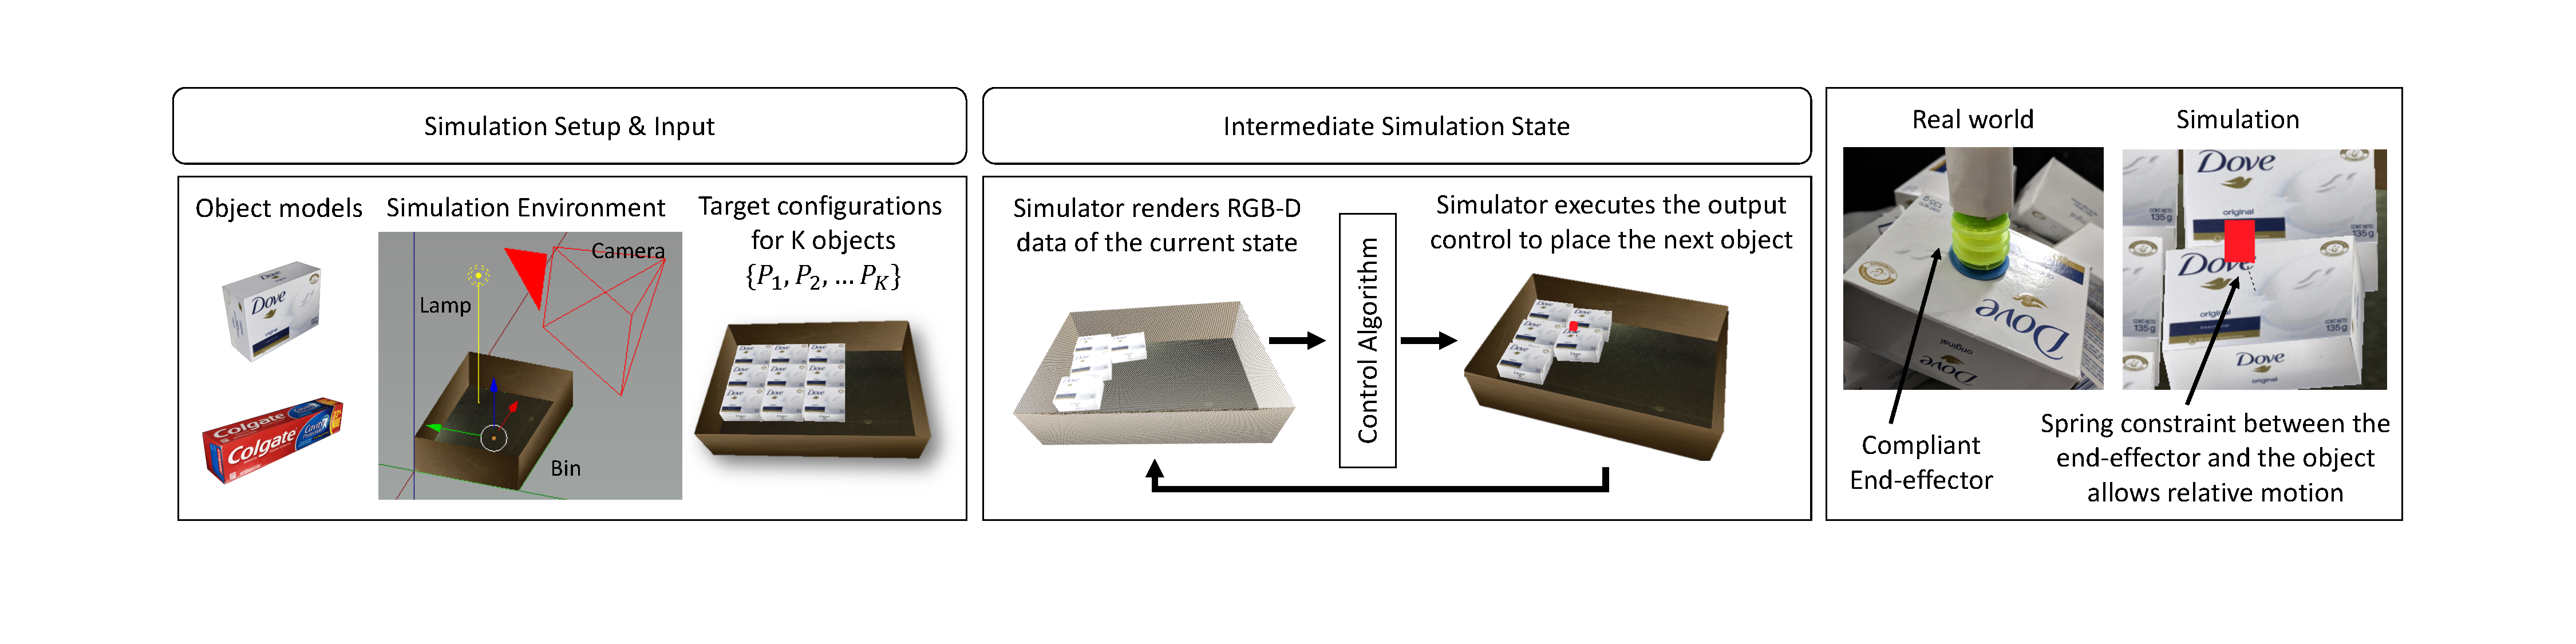
\includegraphics[width=\textwidth]{Figures/simulator.pdf}
\caption{Simulator environment is setup with a bin, lights and camera parameters. Objects are placed sequentially to achieve a desired target configuration. Before each placement, the state of the bin is captured by rendering RGB-D images. The state is provided as input to the control algorithm that computes the motion for the target object. Finally, the controls are executed in the simulator to place the object in the bin. To accurately model the compliance of the real-world end-effector, a spring constraint is applied in simulation between the end-effector and the object. The constraint allows small relative motion and prevents unrealistic collision and jumping of objects that are often observed in rigid-body simulation.}
\label{fig:simulator}
\end{figure*}

